\documentclass{article}
\usepackage{tikz}
\usetikzlibrary{arrows.meta}

\begin{document}

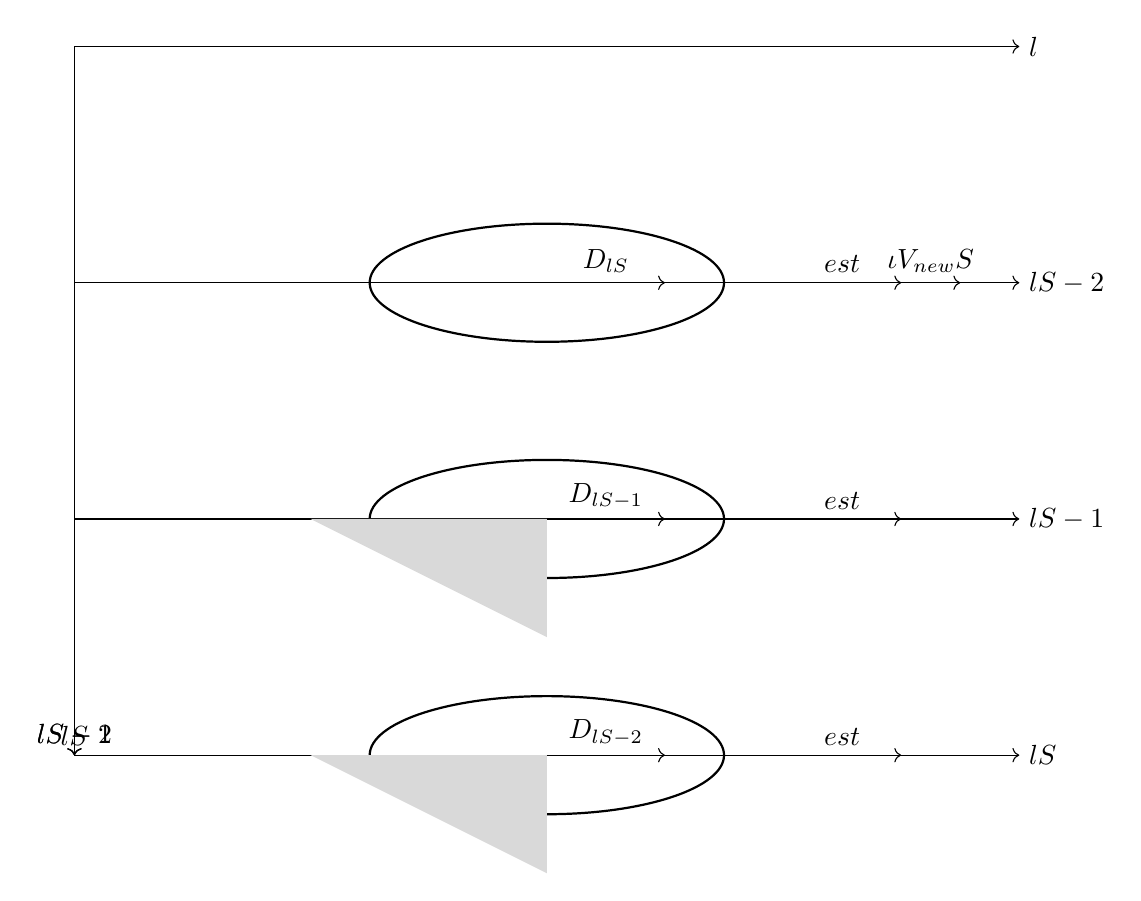
\begin{tikzpicture}[scale=1.5]
    % Draw the horizontal lines
    \draw[->] (0,0) -- (8,0) node[right] {$l$};
    \draw[->] (0,-2) -- (8,-2) node[right] {$lS-2$};
    \draw[->] (0,-4) -- (8,-4) node[right] {$lS-1$};
    \draw[->] (0,-6) -- (8,-6) node[right] {$lS$};

    % Draw the vertical lines
    \draw[->] (0,0) -- (0,-6) node[above] {$lS$};
    \draw[->] (0,-2) -- (0,-6) node[above] {$lS-1$};
    \draw[->] (0,-4) -- (0,-6) node[above] {$lS-2$};

    % Draw the ellipses
    \draw[thick] (4,-2) ellipse (1.5 and 0.5);
    \draw[thick] (4,-4) ellipse (1.5 and 0.5);
    \draw[thick] (4,-6) ellipse (1.5 and 0.5);

    % Draw the shaded triangles
    \fill[gray!30] (2,-4) -- (4,-4) -- (4,-5) -- cycle;
    \fill[gray!30] (2,-6) -- (4,-6) -- (4,-7) -- cycle;

    % Draw the arrows and labels
    \draw[->] (4,-2) -- (5,-2) node[midway,above] {$D_{lS}$};
    \draw[->] (4,-4) -- (5,-4) node[midway,above] {$D_{lS-1}$};
    \draw[->] (4,-6) -- (5,-6) node[midway,above] {$D_{lS-2}$};

    % Draw the "est" labels
    \draw[->] (6,-2) -- (7,-2) node[midway,above] {$est$};
    \draw[->] (6,-4) -- (7,-4) node[midway,above] {$est$};
    \draw[->] (6,-6) -- (7,-6) node[midway,above] {$est$};

    % Draw the "VnewS" label
    \draw[->] (7,-2) -- (7.5,-2) node[midway,above] {$\iota V_{new}S$};
\end{tikzpicture}

\end{document}